% 图片使用了subfigure环境
% 表格都改为了 lstlisting环境
% 协整部分增加了解释
% 本节中所有的英文标点替换为中文标点
% 修正了其它的一些小错误

\section{与退休养老资产的协整关系}
由于美国FOF基金的兴起, 主要源于养老金市场的发展。 美国雇员逐渐选择将养老金计划由DB(Defined Benefit) Plan转向DC(Defined Contribute) Plan, 增大了养老金投资着的投资需求。 而FOF基金作为一种收益稳定、风险二次分散的基金, 自然受到了这些被动投资者的青睐。 下面, 利用彭博数据库中FOF基金资产总量和养老金资产总量的季度数据, 对FOF基金市场与养老金市场进行协整分析。 在2007--2016十年中, 二者的绝对数量和增长率变化趋势如图~\ref{fig:3-0}~:


\begin{figure}[ht]
 \centering
 \subfigure[资产数量]{
   \label{fig:3-0-1} %% label for first subfigure
   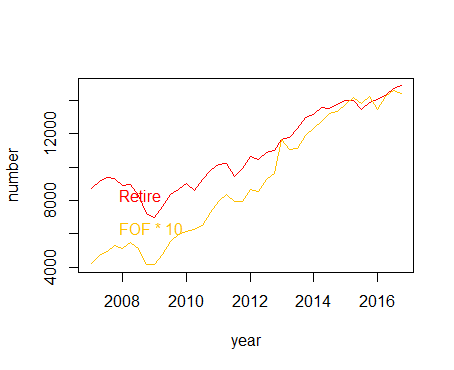
\includegraphics[width=0.45\textwidth]{pic/3-0-1.png}}
 \hspace{1in}
 \subfigure[资产增长率]
   \label{fig:3-0-2} %% label for second subfigure
   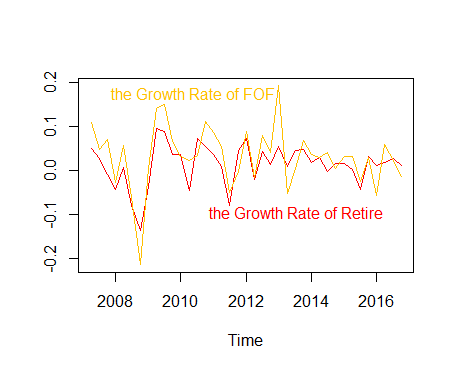
\includegraphics[width=0.45\textwidth]{pic/3-0-2.png}}
 \caption{2007-2016年FOF基金和养老金发展情况季度数据}
 \label{fig:3-0} %% label for entire figure
\end{figure}

% 单位根检验部分
对${FOF_t}$和${Retire_t}$序列分别进行单位根检验。ADF检验和Phillips–Perron的结果接受了原假设(单位根过程), 并且Kwiatkowski–Phillips–Schmidt–Shin检验结果拒绝了原假设(平稳过程)。 因此可以认为${FOF_t}$和${Retire_t}$是非平稳序列。
继续对它们的差分序列${\Delta FOF_t}$和${\Delta Retire_t}$进行单位根检验(表~\ref{tb:3-adf}~), 得到的结果表明它们是平稳序列。 所以, ${FOF_t}$和${Retire_t}$分别是2个$I(1)$序列。下面对这两个序列进行协整估计。

% 单位根检验表格
\begin{lstlisting}
    \begin{table}[]
        \centering
        \caption{单位根检验}
        \label{tb:3-adf}
            \begin{tabular}{l | lll}    \hline \hline
            TEST Method     & ADF   & KPSS & PP    \\ \hline
            FOF             & 2.53  & 1.07 & -0.16 \\
            diff(FOF)       & -3.4  & 0.11 & 40    \\
            Retire          & 1.64  & 1.01 & 0.23  \\
            diff(Retire)    & -2.31 & 0.18 & 1.55  \\ \hline
            10pct           & -1.61 & 0.35 & *     \\
            5pct            & -1.95 & 0.46 & 0.26  \\
            1pct            & -2.62 & 0.74 & *     \\  \hline \hline
            \end{tabular}
    \end{table}
\end{lstlisting}

% 协整部分
首先, 使用最小二乘法估计如下方程:
$$FOF_t = \alpha + \beta \cdot Retire_t + \mu_t$$
得到$\alpha$和$\beta$的估计量$\hat{\alpha}$和$\hat{\beta}$。 估计结果如表~\ref{tab:coin-OLS-estimate}~所示。

% OLS回归结果表格
\begin{lstlisting}
    \begin{table}[ht]
        \centering
        \caption{OLS估计量}
        \label{tab:coin-OLS-estimate}
        \begin{tabular}{l | rrrr}  \hline \hline
            Coefficients: & Estimate   & Std. Error & t value & Pr(\textgreater|t|) \\  \hline
            (Intercept)   & -7.552e+02 & 5.632e+01  & -13.41  & 5.51e-16***        \\
            Retire        & 1.524e-01  & 5.042e-03  & 30.22   & \textless 2e-16***  \\ \hline \hline
        \end{tabular}
    \end{table}
\end{lstlisting}


对残差估计序列${\hat{\mu}_t}$进行单位根检验, ${\hat{\mu}_t}$在ADF检验和PP检验中拒绝了存在单位根的原假设, 在KPSS检验中接受了序列平稳的原假设。因此可以认为${FOF_t}$和${Retire_t}$两个$I(1)$过程得到了平稳的$I(0)$
过程。 即两个序列之间存在着长期的均衡关系(协整关系)。 协整向量为$(1, -0.15)$, 表~\ref{tab:coin-OLS-resid-uniroot}~所示。

% 残差具有平稳性
\begin{lstlisting}
    \begin{table}[ht]
        \centering
        \caption{OLS估计残差的单位根检验}
        \label{tab:coin-OLS-resid-uniroot}
        \begin{tabular}{l | cccc}  \hline \hline
            Tests        & ADF-Test       & KPSS-Test      & PP-Test               \\  \hline
            Statistics   & -3.1799 (<1pct) & 0.2674(<10pct) & -10.0379 (<Z-tau)     \\  \hline \hline
        \end{tabular}
    \end{table}
\end{lstlisting}

% Error Correction Model
记$y_t = FOF_t$, $x_t = Retire_t$, 建立误差修正模型。 由于使用的是季度数据, 所以加入$\Delta y_t$的1--4阶滞后项。
$$
\Delta y_t = \alpha_1 \cdot \Delta y_{t-1} + \alpha_2  \cdot \Delta  y_{t-2} + \alpha_3 \cdot \Delta  y_{t-3} + \alpha_4 \cdot \Delta  y_{t-4} + \beta_0 \cdot \Delta  x_t+\beta_1 \cdot \Delta  x_{t-1} + \gamma \cdot ( y_{t-1}-kx_{t-1}) + \epsilon_t
$$


估计结果表~\ref{tab:coin-correction-model}~所示。

% 误差修正模型的估计结果
\begin{lstlisting}
    \begin{table}[ht]
        \centering
        \caption{误差修正模型估计结果}
        \label{tab:coin-correction-model}
        \begin{tabular}{l | rrrr} \hline \hline
            Coefficients: & Estimate & Std. Error & t value & Pr(\textgreater|t|) \\  \hline
            (Intercept)   & 22.13335 & 11.14436   & 1.986   & 0.0573              \\
            L($\Delta y$, 1)       & -0.46108 & 0.19994    & -2.306  & 0.029*             \\
            L($\Delta y$, 2)       & -0.01601 & 0.12908    & -0.124  & 0.9022              \\
            L($\Delta y$, 3)       & -0.03563 & 0.12999    & -0.274  & 0.7861              \\
            L($\Delta y$, 4)       & -0.02875 & 0.13862    & -0.207  & 0.8373              \\
            L($\Delta x$, 1)       & 0.05842  & 0.02549    & 2.292   & 0.03*              \\
            L($\Delta x$, 0)       & 0.09517  & 0.01852    & 5.138   & 0.000021***        \\
            L(r, 1)                & -0.38373 & 0.16855    & -2.277  & 0.0309*           \\ 
            \hline \hline
        \end{tabular}
    \end{table}
\end{lstlisting}

协整方程的估计结果为
$$\Delta y_t =22.13  -0.46 \cdot \Delta y_{t-1} -0.01 \cdot \Delta  y_{t-2}   -0.04 \cdot \Delta  y_{t-3}  -0.03 \cdot \Delta  y_{t-4} + 0.10 \cdot \Delta  x_t+ 0.06 \cdot \Delta  x_{t-1} -0.38 \cdot ( y_{t-1}-0.15x_{t-1}) + \epsilon_t$$
$\Delta y$的滞后项中,只有一期滞后项是显著的;误差修正项的系数为-0.38,在10\%的程度显著,符合反向修正机制。 协整向量为$(1, -0.15)$。
ECM模型说明FOF基金市场和养老金市场存在长期的稳定关系~\ref{fg:coin-result}~。从资产数量的角度上,养老金市场的发展推动了FOF基金市场的发展;长期均衡中,FOF基金的资产总量维持在养老金市场资产总量的15\%。而上一期的不均衡误差对当期以38\%的比率进行修正。

\begin{figure}[ht]
  \centering
  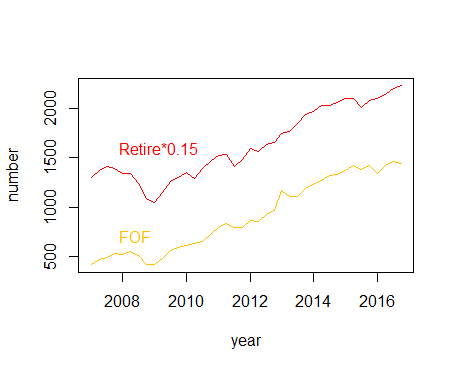
\includegraphics[width=0.6\textwidth]{pic/coin-result.png}
  \caption{长期均衡关系}\label{fg:coin-result}
\end{figure}

美国养老金体系包括政府主办的退休金保险、雇主资助的私营养老金、个人储蓄多个层次。从DB Plan(确定收益计划)到DC Plan(确定退休金计划)的演变,使得雇员更多地考虑到投资工具的收益的稳定性。
而共同基金,特别是FOF是养老金的理想投资工具。和其它投资工具相比,FOF基金具有一些天然的投资优势:(1)低风险性,基金本身通过组合的方式,对股票和证券进行了资产分散;而FOF基金则通过投资不同类型基金,进行双重的风险分散,从而能够获得更加稳定的收益;(2)降低了多样化投资门槛,投资者不再需要繁复地挑选基金,可以通过只投资一个产品来获得相似的投资效果。

借鉴美国养老金与FOF市场的关联关系的实证经验,可以对中国市场得到启示。2016年末,中国社保基金资产总额达到20,423.28亿元。而中国社会提前进入老龄化社会,使得养老保险制度面临更大的挑战。
目前,中国资本市场还不成熟, 特别是股票市场波动较大,存在着资产质量报告及信息不对称、庄家操纵股价等一系列的问题 ,而且缺乏有效的避险工具。在这样的情况下,选择稳定收益的投资工具十分重要。
此外,由美国市场的经验,养老金市场的发展也在推动了FOF基金的发展。养老金成熟的投资于FOF基金,也会促进FOF基金的发展,进而推动共同基金市场的发展。
